\documentclass[a4paper,11pt]{article}
\usepackage[utf8]{inputenc}\usepackage[T1]{fontenc}
\usepackage[english]{babel}\usepackage{lmodern}\usepackage{microtype}
\usepackage{amsmath,amssymb}\usepackage{geometry}
\geometry{a4paper,left=2.2cm,right=2.2cm,top=2.0cm,bottom=2.0cm}
\usepackage{booktabs,array}\usepackage{xcolor}
\definecolor{bokug}{RGB}{0,135,60}\usepackage{tikz}
\usetikzlibrary{arrows.meta,calc}
\usepackage{fancyhdr}\pagestyle{fancy}
\renewcommand{\headrulewidth}{0.4pt}
\usepackage{enumitem}\setlength{\parindent}{0pt}\setlength{\parskip}{4pt}

\begin{document}
\fancyhead[L]{\small VU Mechanik – LAWI 100515 (PI)}\fancyhead[R]{\small SS 2026}\fancyfoot[C]{\thepage}
\begin{center}{\large\bfseries\color{bokug}University of Natural Resources and Life Sciences, Vienna (BOKU)}\\[2pt]{\large\bfseries VU Mechanik – LAWI 100515 (PI)}\\[4pt]Exam \textbf{Group A} \hfill Date: 26.06.2026\\[2pt]\rule{\linewidth}{0.4pt}\end{center}

\begin{center}\textbf{\large Model solution}\end{center}
\begin{center}
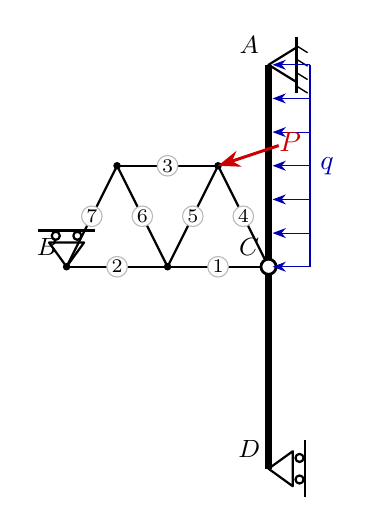
\begin{tikzpicture}[scale=0.855,>=Stealth,line join=round]
  \coordinate (P0) at (0.000,0.000);
  \coordinate (P1) at (0.000,-3.000);
  \coordinate (P2) at (0.000,-6.000);
  \coordinate (TO1) at (-1.500,-3.000);
  \coordinate (TO2) at (-3.000,-3.000);
  \coordinate (TU0) at (-0.750,-1.500);
  \coordinate (TU1) at (-2.250,-1.500);
  \draw[thick] (P1) -- (TO1);
  \draw[thick] (TO1) -- (TO2);
  \draw[thick] (TU0) -- (TU1);
  \draw[thick] (P1) -- (TU0);
  \draw[thick] (TU0) -- (TO1);
  \draw[thick] (TO1) -- (TU1);
  \draw[thick] (TU1) -- (TO2);
  \draw[line width=2.2pt] (P0) -- (P1);
  \draw[line width=2.2pt] (P1) -- (P2);
  \fill (P1) circle (1.6pt);
  \fill (TO1) circle (1.6pt);
  \fill (TO2) circle (1.6pt);
  \fill (TU0) circle (1.6pt);
  \fill (TU1) circle (1.6pt);
  \draw[fill=white,line width=1pt] (P1) circle (3.2pt);
  \draw[thick] (0.000,0.000) -- (0.420,-0.260) -- (0.420,0.260) -- cycle;
  \draw[line width=1pt] (0.420,-0.420) -- (0.420,0.420);
  \draw[line width=0.5pt] (0.420,-0.320) -- (0.580,-0.420);
  \draw[line width=0.5pt] (0.420,-0.120) -- (0.580,-0.220);
  \draw[line width=0.5pt] (0.420,0.080) -- (0.580,-0.020);
  \draw[line width=0.5pt] (0.420,0.280) -- (0.580,0.180);
  \draw[thick] (0.000,-6.000) -- (0.360,-6.260) -- (0.360,-5.740) -- cycle;
  \draw[thick] (0.460,-6.160) circle (0.06) (0.460,-5.840) circle (0.06);
  \draw[line width=1pt] (0.540,-6.420) -- (0.540,-5.580);
  \draw[thick] (-3.000,-3.000) -- (-2.740,-2.640) -- (-3.260,-2.640) -- cycle;
  \draw[thick] (-2.840,-2.540) circle (0.06) (-3.160,-2.540) circle (0.06);
  \draw[line width=1pt] (-2.580,-2.460) -- (-3.420,-2.460);
  \node[circle,fill=white,draw=gray!55,inner sep=0.5pt,font=\scriptsize] at (-0.750,-3.000) {1};
  \node[circle,fill=white,draw=gray!55,inner sep=0.5pt,font=\scriptsize] at (-2.250,-3.000) {2};
  \node[circle,fill=white,draw=gray!55,inner sep=0.5pt,font=\scriptsize] at (-1.500,-1.500) {3};
  \node[circle,fill=white,draw=gray!55,inner sep=0.5pt,font=\scriptsize] at (-0.375,-2.250) {4};
  \node[circle,fill=white,draw=gray!55,inner sep=0.5pt,font=\scriptsize] at (-1.125,-2.250) {5};
  \node[circle,fill=white,draw=gray!55,inner sep=0.5pt,font=\scriptsize] at (-1.875,-2.250) {6};
  \node[circle,fill=white,draw=gray!55,inner sep=0.5pt,font=\scriptsize] at (-2.625,-2.250) {7};
  \draw[->,blue!70!black] (0.620,0.000) -- (0.060,0.000);
  \draw[->,blue!70!black] (0.620,-0.500) -- (0.060,-0.500);
  \draw[->,blue!70!black] (0.620,-1.000) -- (0.060,-1.000);
  \draw[->,blue!70!black] (0.620,-1.500) -- (0.060,-1.500);
  \draw[->,blue!70!black] (0.620,-2.000) -- (0.060,-2.000);
  \draw[->,blue!70!black] (0.620,-2.500) -- (0.060,-2.500);
  \draw[->,blue!70!black] (0.620,-3.000) -- (0.060,-3.000);
  \draw[blue!70!black,thick] (0.620,0.000) -- (0.620,-3.000);
  \node[blue!70!black] at (0.870,-1.500) {$q$};
  \draw[->,red!80!black,line width=1.1pt] (0.151,-1.200) -- (-0.750,-1.500);
  \node[red!80!black] at (0.322,-1.143) {$P$};
  \node[font=\small] at (0.000,0.000) [xshift=-7pt,yshift=7pt] {$A$};
  \node[font=\small] at (0.000,-3.000) [xshift=-7pt,yshift=7pt] {$C$};
  \node[font=\small] at (0.000,-6.000) [xshift=-7pt,yshift=7pt] {$D$};
  \node[font=\small] at (-3.000,-3.000) [xshift=-7pt,yshift=7pt] {$B$};
\end{tikzpicture}
\end{center}
\par\medskip\textbf{1.\ Static determinacy}\par Counting criterion $n=3k-(a+z)$ (bodies $k$, reactions $a$, interaction forces $z$):
\[ n=3k-(a+z)=3\cdot2-(4+2)=0\ \Rightarrow\ \text{statically determinate} \]
\par\medskip\textbf{2.\ Support reactions and hinge forces}\par
$A:\ R_x=14.25,\ R_y=-3.75$\quad $D:\ R_x=9.75,\ R_y=0$\quad $B:\ R_x=0,\ R_y=8.75$\par $C:\ H_x=-15,\ H_y=3.75$
\par\medskip\textbf{3.\ Truss member forces}\par
\begin{center}\renewcommand{\arraystretch}{1.1}\begin{tabular}{c r l}
\toprule
Member & Force $S$ [kN] & Type \\
\midrule
  1 & 13.12 & tension \\
  2 & 4.38 & tension \\
  3 & -8.75 & compression \\
  4 & 4.19 & tension \\
  5 & -9.78 & compression \\
  6 & 9.78 & tension \\
  7 & -9.78 & compression \\
\bottomrule
\end{tabular}\end{center}
\begin{center}
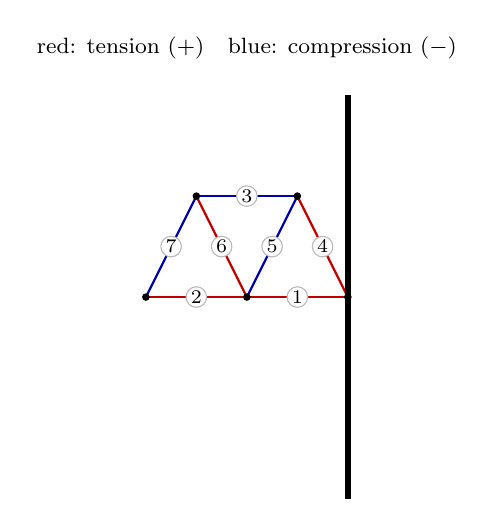
\begin{tikzpicture}[scale=0.855,>=Stealth,line join=round]
  \coordinate (P0) at (0.000,0.000);
  \coordinate (P1) at (0.000,-3.000);
  \coordinate (P2) at (0.000,-6.000);
  \coordinate (TO1) at (-1.500,-3.000);
  \coordinate (TO2) at (-3.000,-3.000);
  \coordinate (TU0) at (-0.750,-1.500);
  \coordinate (TU1) at (-2.250,-1.500);
  \draw[thick,red!75!black] (P1) -- (TO1);
  \draw[thick,red!75!black] (TO1) -- (TO2);
  \draw[thick,blue!70!black] (TU0) -- (TU1);
  \draw[thick,red!75!black] (P1) -- (TU0);
  \draw[thick,blue!70!black] (TU0) -- (TO1);
  \draw[thick,red!75!black] (TO1) -- (TU1);
  \draw[thick,blue!70!black] (TU1) -- (TO2);
  \draw[line width=2pt] (P0) -- (P1);
  \draw[line width=2pt] (P1) -- (P2);
  \fill (P1) circle (1.6pt);
  \fill (TO1) circle (1.6pt);
  \fill (TO2) circle (1.6pt);
  \fill (TU0) circle (1.6pt);
  \fill (TU1) circle (1.6pt);
  \node[circle,fill=white,draw=gray!55,inner sep=0.5pt,font=\scriptsize] at (-0.750,-3.000) {1};
  \node[circle,fill=white,draw=gray!55,inner sep=0.5pt,font=\scriptsize] at (-2.250,-3.000) {2};
  \node[circle,fill=white,draw=gray!55,inner sep=0.5pt,font=\scriptsize] at (-1.500,-1.500) {3};
  \node[circle,fill=white,draw=gray!55,inner sep=0.5pt,font=\scriptsize] at (-0.375,-2.250) {4};
  \node[circle,fill=white,draw=gray!55,inner sep=0.5pt,font=\scriptsize] at (-1.125,-2.250) {5};
  \node[circle,fill=white,draw=gray!55,inner sep=0.5pt,font=\scriptsize] at (-1.875,-2.250) {6};
  \node[circle,fill=white,draw=gray!55,inner sep=0.5pt,font=\scriptsize] at (-2.625,-2.250) {7};
  \node[font=\footnotesize] at (-1.50,0.70) {red: tension $(+)$\quad blue: compression $(-)$};
\end{tikzpicture}
\end{center}
\par\medskip\textbf{4.\ Section-force diagrams of the beams}\par
\begin{center}
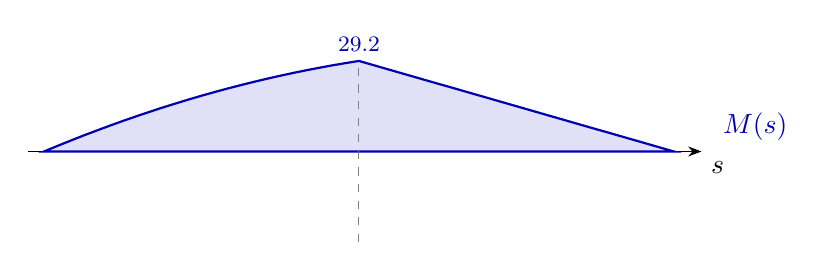
\begin{tikzpicture}[>=Stealth]
  \draw[->] (-0.2,0) -- (8.35,0) node[below right]{$s$};
  \filldraw[fill=blue!70!black!12,draw=blue!70!black,thick] (0,0) -- plot coordinates {(0.000,0.000) (0.167,0.069) (0.333,0.136) (0.500,0.202) (0.667,0.265) (0.833,0.327) (1.000,0.387) (1.167,0.445) (1.333,0.501) (1.500,0.556) (1.667,0.608) (1.833,0.659) (2.000,0.708) (2.167,0.755) (2.333,0.800) (2.500,0.843) (2.667,0.885) (2.833,0.924) (3.000,0.962) (3.167,0.998) (3.333,1.032) (3.500,1.064) (3.667,1.095) (3.833,1.123) (4.000,1.150) (4.000,1.150) (4.167,1.102) (4.333,1.054) (4.500,1.006) (4.667,0.958) (4.833,0.910) (5.000,0.862) (5.167,0.815) (5.333,0.767) (5.500,0.719) (5.667,0.671) (5.833,0.623) (6.000,0.575) (6.167,0.527) (6.333,0.479) (6.500,0.431) (6.667,0.383) (6.833,0.335) (7.000,0.287) (7.167,0.240) (7.333,0.192) (7.500,0.144) (7.667,0.096) (7.833,0.048) (8.000,0.000)} -- (8.000,0) -- cycle;
  \draw[gray,dashed,thin] (4.000,-1.15) -- (4.000,1.15);
  \node[above,blue!70!black,font=\footnotesize] at (4.000,1.150) {29.2};
  \node[blue!70!black,right] at (8.50,0.32) {$M(s)$};
\end{tikzpicture}\\[5pt]
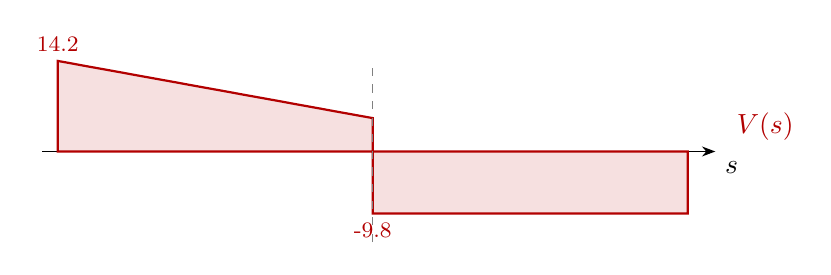
\begin{tikzpicture}[>=Stealth]
  \draw[->] (-0.2,0) -- (8.35,0) node[below right]{$s$};
  \filldraw[fill=red!70!black!12,draw=red!70!black,thick] (0,0) -- plot coordinates {(0.000,1.150) (0.167,1.120) (0.333,1.089) (0.500,1.059) (0.667,1.029) (0.833,0.999) (1.000,0.968) (1.167,0.938) (1.333,0.908) (1.500,0.878) (1.667,0.847) (1.833,0.817) (2.000,0.787) (2.167,0.757) (2.333,0.726) (2.500,0.696) (2.667,0.666) (2.833,0.636) (3.000,0.605) (3.167,0.575) (3.333,0.545) (3.500,0.514) (3.667,0.484) (3.833,0.454) (4.000,0.424) (4.000,-0.787) (4.167,-0.787) (4.333,-0.787) (4.500,-0.787) (4.667,-0.787) (4.833,-0.787) (5.000,-0.787) (5.167,-0.787) (5.333,-0.787) (5.500,-0.787) (5.667,-0.787) (5.833,-0.787) (6.000,-0.787) (6.167,-0.787) (6.333,-0.787) (6.500,-0.787) (6.667,-0.787) (6.833,-0.787) (7.000,-0.787) (7.167,-0.787) (7.333,-0.787) (7.500,-0.787) (7.667,-0.787) (7.833,-0.787) (8.000,-0.787)} -- (8.000,0) -- cycle;
  \draw[gray,dashed,thin] (4.000,-1.15) -- (4.000,1.15);
  \node[above,red!70!black,font=\footnotesize] at (0.000,1.150) {14.2};
  \node[below,red!70!black,font=\footnotesize] at (4.000,-0.787) {-9.8};
  \node[red!70!black,right] at (8.50,0.32) {$V(s)$};
\end{tikzpicture}\\[5pt]
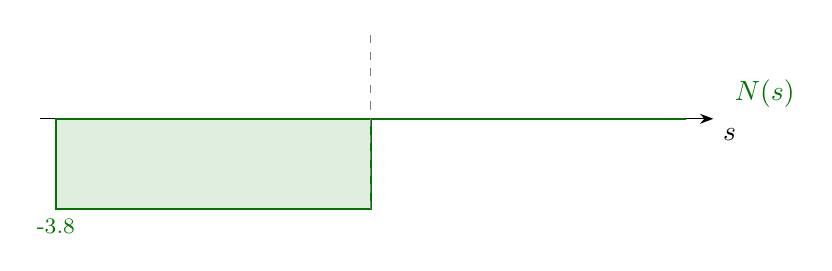
\begin{tikzpicture}[>=Stealth]
  \draw[->] (-0.2,0) -- (8.35,0) node[below right]{$s$};
  \filldraw[fill=green!45!black!12,draw=green!45!black,thick] (0,0) -- plot coordinates {(0.000,-1.150) (0.167,-1.150) (0.333,-1.150) (0.500,-1.150) (0.667,-1.150) (0.833,-1.150) (1.000,-1.150) (1.167,-1.150) (1.333,-1.150) (1.500,-1.150) (1.667,-1.150) (1.833,-1.150) (2.000,-1.150) (2.167,-1.150) (2.333,-1.150) (2.500,-1.150) (2.667,-1.150) (2.833,-1.150) (3.000,-1.150) (3.167,-1.150) (3.333,-1.150) (3.500,-1.150) (3.667,-1.150) (3.833,-1.150) (4.000,-1.150) (4.000,0.000) (4.167,0.000) (4.333,0.000) (4.500,0.000) (4.667,0.000) (4.833,0.000) (5.000,0.000) (5.167,0.000) (5.333,0.000) (5.500,0.000) (5.667,0.000) (5.833,0.000) (6.000,0.000) (6.167,0.000) (6.333,0.000) (6.500,0.000) (6.667,0.000) (6.833,0.000) (7.000,0.000) (7.167,0.000) (7.333,0.000) (7.500,0.000) (7.667,0.000) (7.833,0.000) (8.000,0.000)} -- (8.000,0) -- cycle;
  \draw[gray,dashed,thin] (4.000,-1.15) -- (4.000,1.15);
  \node[below,green!45!black,font=\footnotesize] at (0.000,-1.150) {-3.8};
  \node[green!45!black,right] at (8.50,0.32) {$N(s)$};
\end{tikzpicture}\\[10pt]
\end{center}
\end{document}